%%%%%%%%%%%%%%%%%%%%%%%%%%%%%%%%%%%%%%%%%%%%%%%%%%%%%%%%%%%%%%%%%%%%%%%%%%%%%%%%%%%%%%%%%%%%%%%%%%%%%%%%%%%%%%%%%%%%%%%%%%%%%%%%
%%%%%%%%%%%%%% Artigo SMN-Q - Sistema de Monitoramento e Notificação de Eventos de Queda em Pacientes Idosos                   %%
%%%%%%%%%%%%%%%%%%%%%%%%%%%%%%%%%%%%%%%%%%%%%%%%%%%%%%%%%%%%%%%%%%%%%%%%%%%%%%%%%%%%%%%%%%%%%%%%%%%%%%%%%%%%%%%%%%%%%%%%%%%%%%%%

\section{\esp Introdução}

Quedas em idosos são um dos maiores problemas de saúde pública envolvendo essa faixa etária. De acordo com a \citeonline{who2018}, ocorrem cerca de 646 mil mortes por queda todo ano no mundo, e idosos acima de 65 anos são as principais vítimas. No Brasil, \citeonline{cunha2014} relata que aproximadamente 40 mil idosos morrem anualmente em decorrência de quedas, com taxa de mortalidade seis vezes maior entre os maiores de 80 anos. O tempo que a pessoa permanece no chão sem socorro --- o chamado \textit{long lie} --- agrava o quadro, especialmente quando o idoso vive sozinho.

As soluções comerciais existentes cobram entre R\$ 150,00 e R\$ 300,00 por mês, valor inviável para grande parte da população idosa brasileira. Este trabalho propõe o SMN-Q (Sistema de Monitoramento e Notificação de Eventos de Queda), um protótipo físico de baixo custo baseado no microcontrolador ESP32-C3 e em acelerômetro tri-axial, com o objetivo de detectar quedas e notificar um cuidador em tempo real por meio de comunicação sem fio. O projeto se alinha aos Objetivos de Desenvolvimento Sustentável 3 (Saúde e Bem-Estar) e 10 (Redução das Desigualdades).

Este trabalho evolui uma versão anterior, validada em ambiente de simulação (Tinkercad), migrando o sistema para hardware físico real e incorporando duas melhorias substanciais: um algoritmo de detecção por fases, fiel à literatura, e a notificação efetiva do cuidador via Bluetooth.

\section{\esp Metodologia}

O projeto foi desenvolvido em duas frentes: a montagem do circuito eletrônico físico em protoboard e a implementação do algoritmo em linguagem Arduino/C++. Os trabalhos de \citeonline{vieira2019} e \citeonline{cabral2022} serviram como referência para o cálculo da magnitude resultante da aceleração, para a lógica de detecção por fases e para o uso do filtro de média móvel.

\subsection{\esp Componentes do circuito}

O sistema é construído em torno do microcontrolador ESP32-C3 Super Mini, escolhido por integrar conectividade sem fio (Bluetooth e Wi-Fi) em um encapsulamento compacto, adequado a um dispositivo de uso vestível. O circuito conta com três entradas: o acelerômetro MPU6050 (sensor digital tri-axial, comunicação via barramento I2C), um potenciômetro para seleção do modo de operação e um botão para cancelamento ou pânico. As saídas são um LED RGB para feedback visual, um buzzer para alarme sonoro e um display LCD 16x2 (com módulo I2C) para mensagens.

\subsection{\esp Diagrama de ligações}

O acelerômetro MPU6050 e o display LCD compartilham o mesmo barramento I2C (pinos SDA e SCL), operando em endereços distintos (0x68 e 0x27, respectivamente), o que reduz a quantidade de ligações. A Tabela \ref{tab:pinagem} detalha a pinagem completa do circuito, e a Figura \ref{fig:circuito} apresenta o protótipo montado em protoboard.

\begin{table}[H]
\centering
\footnotesize
\caption{Mapeamento de ligações dos componentes ao ESP32-C3}
\label{tab:pinagem}
\begin{tabular}{|l|l|l|}
\hline
\textbf{Componente} & \textbf{Pino do componente} & \textbf{Pino do ESP32-C3} \\
\hline
\multirow{4}{*}{MPU6050 (acelerômetro)} & VCC & 3,3V \\
 & GND & GND \\
 & SDA & GPIO8 \\
 & SCL & GPIO9 \\
\hline
\multirow{4}{*}{Display LCD I2C} & VCC & 3,3V \\
 & GND & GND \\
 & SDA & GPIO8 (compartilhado) \\
 & SCL & GPIO9 (compartilhado) \\
\hline
\multirow{2}{*}{Potenciômetro} & Terminal central & GPIO4 \\
 & Terminais laterais & 3,3V e GND \\
\hline
\multirow{4}{*}{LED RGB} & Pino R (via resistor) & GPIO3 \\
 & Pino G (via resistor) & GPIO5 \\
 & Pino B (via resistor) & GPIO6 \\
 & Terminal comum & GND \\
\hline
\multirow{2}{*}{Buzzer} & Terminal positivo & GPIO10 \\
 & Terminal negativo & GND \\
\hline
\multirow{2}{*}{Botão} & Terminal 1 & GPIO2 \\
 & Terminal 2 & GND \\
\hline
\end{tabular}
\end{table}

\begin{figure}[H]
    \centering
    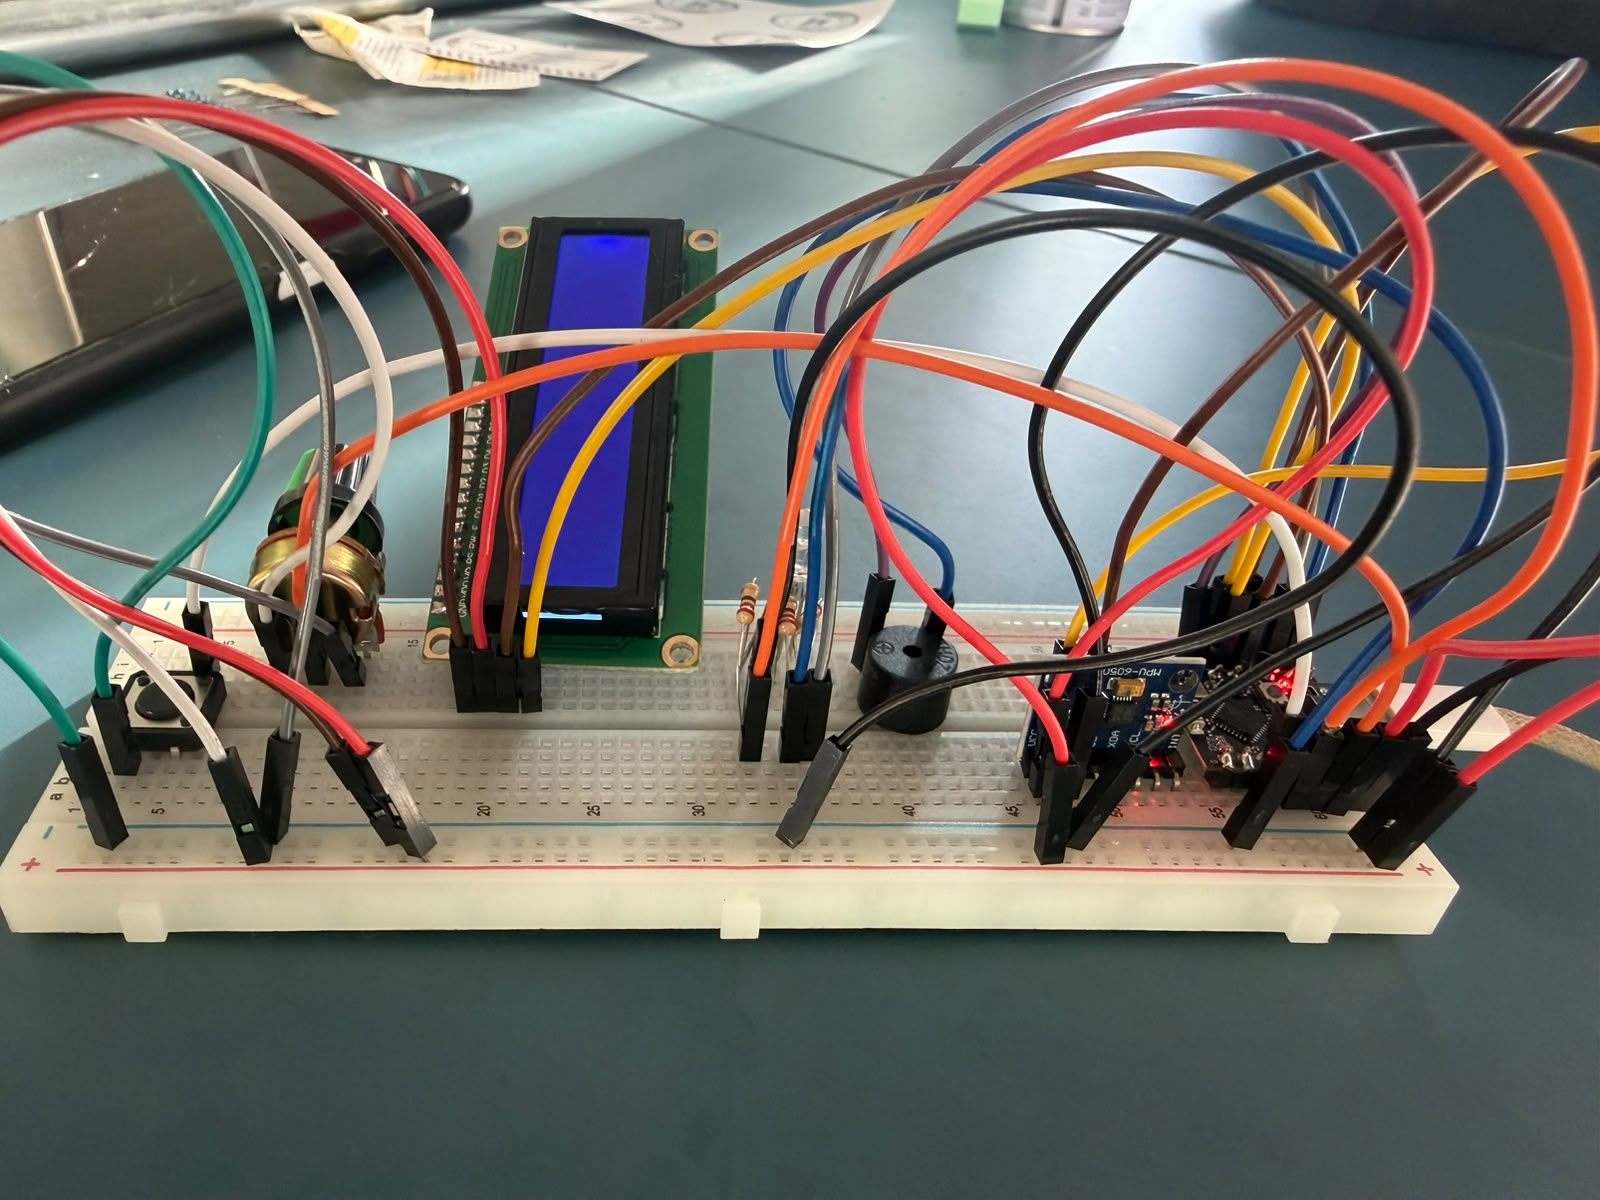
\includegraphics[width=0.85\textwidth]{figuras/protoboard.jpeg}
    \caption{Protótipo do SMN-Q montado em protoboard.}
    \label{fig:circuito}
\end{figure}

A alimentação, durante a validação, foi realizada por cabo USB; para operação portátil, o projeto prevê alimentação por bateria de íon-lítio 18650 com módulos de carga (TP4056) e elevação de tensão (MT3608).

\subsection{\esp Algoritmo de detecção}

A cada 50 ms o sistema lê os três eixos do acelerômetro e calcula a magnitude resultante da aceleração (Equação \ref{eq:magnitude}), expressa em unidades de gravidade (g).

\begin{equation}
\label{eq:magnitude}
Norm(x, y, z) = \sqrt{x^{2} + y^{2} + z^{2}}
\end{equation}

A abordagem de detecção adotada é baseada em fases, seguindo o padrão descrito pela literatura. Uma queda real apresenta uma assinatura característica composta por dois eventos em sequência: primeiro a queda livre, na qual a magnitude da aceleração cai para valores próximos de zero (abaixo de 0,6g), quando o corpo em queda deixa de sentir a força gravitacional plena; e, em seguida, o impacto, no qual a magnitude apresenta um pico acentuado (acima de 2,5g) no momento em que o corpo atinge o solo. O sistema somente confirma uma queda quando ambos os eventos ocorrem em sequência, dentro de uma janela temporal de aproximadamente 1,2 segundo.

Essa estratégia de duas fases torna a detecção robusta a mudanças de orientação do dispositivo. Movimentos lentos e cotidianos --- como sentar, inclinar-se ou reposicionar o aparelho no bolso --- não completam a sequência queda livre--impacto e, portanto, não geram falsos positivos. Diferentemente da abordagem baseada apenas na variação absoluta da magnitude em relação a uma referência fixa, a detecção por fases distingue com maior precisão uma queda real de um simples movimento brusco.

Para o tratamento do sinal, o sistema emprega o filtro de média móvel como recurso de suavização de ruído do sensor. Na etapa de detecção do impacto, contudo, a magnitude instantânea (não filtrada) é utilizada, uma vez que o filtro atenuaria justamente os picos que caracterizam a colisão.

O potenciômetro atua como seletor de modo de operação. No modo REAL, os limiares seguem os valores da literatura (queda livre abaixo de 0,6g e impacto acima de 2,5g), apropriados à detecção de quedas verdadeiras. No modo DEMO, os limiares são reduzidos, permitindo a demonstração controlada do funcionamento do sistema em bancada sem a necessidade de reproduzir um impacto real.

\subsection{\esp Notificação sem fio}

Ao confirmar uma emergência, o SMN-Q notifica o cuidador por meio de comunicação sem fio \textit{Bluetooth Low Energy} (BLE). O ESP32-C3 atua como servidor BLE, anunciando um serviço ao qual o \textit{smartphone} do cuidador se conecta. No momento da detecção, o dispositivo transmite mensagens de alerta que são recebidas em tempo real no aparelho móvel, informando a ocorrência da queda e a necessidade de socorro. A escolha do BLE justifica-se pelo baixo consumo energético, característica desejável em um dispositivo de uso contínuo junto ao corpo do usuário.

\subsection{\esp Rotina de teste}

Foi implementada uma rotina acionada pela tecla \verb|t| no Monitor Serial. Ela mostra as leituras de todas as entradas, aciona cada saída em sequência (LED nas quatro cores, buzzer, LCD) e retorna ao estado normal. Adicionalmente, o comando \verb|q| dispara diretamente o ciclo de alerta, facilitando a demonstração do funcionamento sem a necessidade de manipular fisicamente o acelerômetro.

\section{\esp Resultados}

O protótipo atendeu a todos os requisitos técnicos propostos. A Tabela \ref{tab:requisitos} relaciona cada requisito exigido com a respectiva implementação no SMN-Q.

\begin{table}[H]
\centering
\footnotesize
\caption{Requisitos do projeto e respectivo atendimento}
\label{tab:requisitos}
\begin{tabular}{|p{4.2cm}|p{6.8cm}|p{1.8cm}|}
\hline
\textbf{Requisito} & \textbf{Como foi atendido} & \textbf{Situação} \\
\hline
Sensor analógico com ajuste por potenciômetro & Potenciômetro seleciona o modo de operação (REAL/DEMO) e ajusta os limiares de detecção & Atendido \\
\hline
Sensor digital (resolução $>$ 2 bits) com tratamento de sinal & Acelerômetro MPU6050 (I2C) com filtro de média móvel aplicado à magnitude & Atendido \\
\hline
Filtro de média móvel & Implementado sobre a magnitude resultante da aceleração & Atendido \\
\hline
Interface de entrada do usuário & Botão de cancelamento/pânico & Atendido \\
\hline
Pelo menos 3 atuadores de saída & LED RGB, buzzer e display LCD 16x2 & Atendido \\
\hline
Conectividade sem fio (Bluetooth) & Notificação do cuidador via \textit{Bluetooth Low Energy} (BLE) no momento da queda & Atendido \\
\hline
Modularidade do código & Código estruturado em funções específicas (leitura, filtro, detecção, alerta, notificação) & Atendido \\
\hline
Legibilidade e nomenclatura & Nomes de variáveis e funções autoexplicativos em português & Atendido \\
\hline
Documentação/comentários & Trechos complexos comentados, explicando a lógica de detecção & Atendido \\
\hline
Entregável (protótipo físico ou MVP) & Protótipo físico funcional montado em protoboard & Atendido \\
\hline
\end{tabular}
\end{table}

O Algoritmo \ref{alg:ciclo-alerta} apresenta a sequência executada quando o sistema detecta uma possível queda. A janela de 15 segundos para cancelamento permite que o usuário interrompa o alarme em caso de falso positivo --- por exemplo, ao tropeçar e se recuperar sozinho.

\begin{center}
\begin{minipage}[ht]{13cm}
\begin{algorithm}[H]
  \footnotesize
  \caption{Ciclo de Alerta e Emergência}
  \label{alg:ciclo-alerta}
  \begin{algorithmic}[1]
    \STATE \textbf{Entrada:} Sequência de queda livre + impacto detectada pelo acelerômetro
    \STATE \textbf{Saída:} Notificação ao cuidador ou cancelamento
    \STATE Aciona LED amarelo, buzzer de alerta e exibe ``Possível queda detectada'' no LCD
    \STATE Envia alerta preliminar ao cuidador via Bluetooth
    \STATE Inicia contagem regressiva de 15 segundos
    \FOR{$t = 15$ \TO $1$}
        \STATE Exibe $t$ no LCD
        \IF{botão pressionado}
            \STATE Cancela alarme, notifica cancelamento via Bluetooth e retorna ao estado normal
            \STATE \textbf{Retorna}
        \ENDIF
        \STATE Aguarda 1 segundo
    \ENDFOR
    \STATE Aciona LED vermelho, buzzer forte e exibe ``EMERGÊNCIA!'' no LCD
    \STATE Envia notificação de emergência ao cuidador via Bluetooth
  \end{algorithmic}
\end{algorithm}
\end{minipage}
\end{center}

A Figura \ref{fig:fluxograma} apresenta o fluxograma completo do funcionamento do sistema. O LED RGB sinaliza visualmente cada estado: verde para monitoramento normal, azul no instante de detecção da fase de queda livre, amarelo durante o alerta e vermelho na emergência confirmada. Essa codificação por cores facilita o entendimento rápido do que está acontecendo.

\begin{figure}[H]
    \centering
    
\includegraphics[width=\textwidth,height=0.92\textheight,keepaspectratio]{figuras/fluxograma_sistema.png}
    \caption{Fluxograma do funcionamento do sistema SMN-Q.}
    \label{fig:fluxograma}
\end{figure}

A validação física confirmou o funcionamento integrado de todos os subsistemas. A detecção por fases mostrou-se estável e imune a falsos positivos decorrentes de mudanças de orientação do dispositivo. A notificação via Bluetooth foi verificada por meio de um \textit{smartphone} conectado ao sistema, no qual as mensagens de alerta e de emergência foram recebidas em tempo real no momento da detecção.

\section{\esp Conclusão}

O SMN-Q foi implementado fisicamente e cumpriu todos os requisitos técnicos do projeto. O algoritmo de detecção por fases, baseado na sequência de queda livre e impacto, funcionou de forma estável e demonstrou-se mais robusto que a abordagem simplificada da versão anterior, especialmente quanto à imunidade a falsos positivos por mudança de posição do dispositivo. A janela de cancelamento de 15 segundos ajuda a evitar que falsos alarmes incomodem o usuário, e a notificação por Bluetooth concretizou o objetivo de comunicar o cuidador em tempo real.

A implementação física mostrou-se viável e acessível. Utilizando o ESP32-C3 Super Mini e o acelerômetro MPU6050, o custo total estimado fica entre R\$ 200,00 e R\$ 280,00 --- muito abaixo das mensalidades das soluções comerciais. A notificação ao cuidador, hoje realizada via Bluetooth, poderia ser estendida por um \textit{Progressive Web App} (PWA) com Firebase Cloud Messaging, permitindo o alcance remoto por meio de \textit{push notification} pela internet.

Como melhorias futuras, três caminhos parecem promissores: expandir o algoritmo de detecção para as quatro fases propostas por \citeonline{vieira2019}, incorporando também a fase de imobilidade pós-impacto; adicionar a distinção entre quedas bruscas e suaves conforme \citeonline{cabral2022}, capturando também escorregões lentos; e desenvolver a calibração adaptativa personalizada proposta por \citeonline{ren2015}, em que o sistema aprende o padrão de cada usuário ao longo do tempo. Uma calibração de seis pontos do acelerômetro também é sugerida para aumentar a precisão das leituras em qualquer orientação.
